\section{Image Gradients}
\subsection{Calculating Gradients}
The horizontal gradient of the image can be determined using the following formula:

\begin{equation}
    H_x(z_1, z_2) = z_2 - z_2^{-1} 
\end{equation}

\noindent Using the same conventions defined before, we can arrive at the following convolution mask:

\begin{equation}
    H_x = 
    \begin{bmatrix}
        0 & -1 & 0 \\
        0 &  0 & 0 \\
        0 &  1 & 0 \\
    \end{bmatrix}
\end{equation}

\noindent The vertical gradient, similar to the horizontal one, has its own transfer function and therefore a convolution mask can also be derived. The steps of which are shown below.

\begin{gather}
        H_y(z_1, z_2) = z_1 - z_1^{-1} \\
        \quad
        H_x = 
        \begin{bmatrix}
             0 & 0 & 0 \\
            -1 & 0 & 1 \\
             0 & 0 & 0 \\
        \end{bmatrix}
\end{gather}

\noindent These can be convolved with the image using the \textcolor{MATLABBlue}{\lstinline|conv2|} function to produce a gradient map for each axes. A bias of 0.5 was added to each image so that derivative values that are close to 0 would appear gray, while highly negative and positive derivatives would appear black and white respectively. Once the horizontal and vertical derivatives are calculated, we can calculate and plot their magnitude, which had to be rescaled into the range of 0-1. The derivatives and the magnitude can be seen in Figure \ref{fig:ImageGradient} below.

\begin{figure}[!h]
    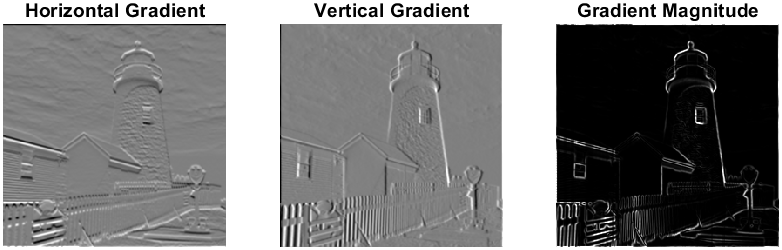
\includegraphics[width=1\textwidth]{ImageGradients.png}
    \centering
    \caption{Horizontal and Vertical Gradients and the Magnitude}
    \label{fig:ImageGradient}
\end{figure}